\section{Methods}
\label{sec:methods}
\label{subsec:methods:overview}

Here we provide a brief overview of the several methods described in this manuscript.
First, we rely on CLAM (Clustered Learning of Approximate Manifolds) as a fairly na\"ive clustering method; CLAM derives from CHESS~\cite{ishaq2019clustered} but introduces significant novelty: while CHESS only clustered to a pre-specified depth for the \emph{sole} purpose of search, CLAM uses a similar clustering on several training sets not included in testing to learn data properties for which anomaly detection will perform well across those datasets.
Unlike CHESS, CLAM does not use a specific depth to halt clustering; instead, it tracks properties including local fractal dimension, cluster cardinality, and moving averages thereof, based upon a training dataset.
The motivation behind these properties is driven by the manifold hypothesis: as the divisive clustering begins to ``separate'' different regions of the manifold, the fractal dimension and cluster cardinality should begin to change; ideally, we seek clusters that optimally ``cover'' the manifold as described in~\cite{yu2015entropy}, though these clusters will clearly not all be at the same depth of the tree across the manifold.
Clustering too deeply will lead to locally uniform-density clusters of \emph{high} fractal dimension, while clustering too shallowly will lead to clusters that contain highly varied regions of the manifold.
We seek to find the optimal balance such that the clusters discover the structure of the manifold.
The stopping criteria are described in Section~\ref{subsubsec:methods:clam:clustering}.
Importantly and novelly, these stopping criteria are not uniform for a given dataset; they are adaptive with differing properties of different regions of the manifold, and may exist at different depths of the tree (see Figure~\ref{fig:methods:graph-generation}).
Also novelly, a graph is induced from the overlap among clusters at this set of depths (see Section~\ref{subsec:methods:induced-graphs}, and this graph informs two of the six anomaly-detection algorithms that CLAM enables (see Section~\ref{subsec:methods:individual-algorithms}).
CLAM relies on an ensemble-learning approach based on six simple heuristics; the ensemble-learning approach is described in Section~\ref{subsec:methods:ensemble}.
These distinct heuristics attempt to encompass distinct notions of what make a datapoint anomalous: is it truly isolated, or is the distribution of datapoints multi-modal, or is it very low-dimensional despite being embedded in a high-dimensional space?

In all, CLAM builds on a clustering algorithm originally developed for a different purpose (accelerated approximate search) and uses a novel graph-inference approach to enable several anomaly-detection heuristics that are effective in practice.


\subsection{CLAM}
\label{subsec:methods:clam}

We present a manifold-mapping algorithm called CLAM (Clustered Learning of Approximate Manifolds).
As input, we need a dataset and a distance function for that dataset.
A dataset is a collection of $n$-points in a $D$-dimensional embedding space, $\textbf{X} = \{x_1 \dots x_n\}, x_i \in \mathbb{R}^D$.
A Distance Function takes two points in the dataset and produces a non-negative real number, $f : (\mathbb{R}^D, \mathbb{R}^D) \mapsto \mathbb{R}^+$.
The distance must be such that $f(x, x) = 0$ and $f(x, y) = f(y, x)$ $\forall x, y \in X$.
The distance function may or may not obey the triangle-inequality.
In this paper we used $L1$-norm and $L2$-norm, which are metrics.
We provide proofs of the complexity of each algorithm in the Supplement.

\subsubsection{Clustering}
\label{subsubsec:methods:clam:clustering}

We start by building a divisive-hierarchical clustering of the data based on a random sampling of $\sqrt k$ points from the  $k$ points in a given cluster from the tree.
This achieves clustering in expected $\mathcal{O}(n \lg n)$ time, giving us a tree of clusters, with the root containing every point in the dataset and each leaf containing a single point from the dataset.
The CLAM clustering algorithm is defined in Algorithm~\ref{alg:clam-partition}.
The procedure is inspired from~\cite{ishaq2019clustered}, although we have improved upon their partition method.
The root-cluster contains all points in the dataset and clusters are recursively partitioned until each leaf-cluster contains only one point.
% We can't cite our work as "us" during the review process

\begin{algorithm} % enter the algorithm environment
\caption{Partition} % give the algorithm a caption
\label{alg:clam-partition} % and a label for \ref{} commands later in the document
\begin{algorithmic}[1] % enter the algorithmic environment
    \REQUIRE $cluster$
    \STATE $k \leftarrow \lfloor \sqrt{|cluster.points|} \rfloor$
    \STATE $seeds \leftarrow k$ random points from $cluster.points$
    \STATE $c \leftarrow$ geometric median of $cluster.points$
    \STATE $r \leftarrow \argmax d(c,x) \ \forall \ x \in cluster.points$
    \STATE $l \leftarrow \argmax d(r,x) \ \forall \ x \in cluster.points$
    \STATE $cluster.left \leftarrow \{x | x \in cluster.points \land d(l,x) \le d(r,x)\}$
    \STATE $cluster.right \leftarrow \{x | x \in cluster.points \land d(r,x) < d(l,x)\}$
    \IF{$|cluster.left| > 1$}
        \STATE Partition(cluster.left)
    \ENDIF
    \IF{$|cluster.right| > 1$}
        \STATE Partition(cluster.right)
    \ENDIF
\end{algorithmic}
\end{algorithm}

These clusters have several interesting and important properties for us to consider.
These include the \textit{cardinality}, the number of points in a cluster;
\textit{center}, the geometric median of points contained in a cluster;
\textit{radius}, the distance to the farthest point from the center;
and \textit{local fractal dimension},
as given by:

\begin{gather}
    \log_2\bigg(\frac{|B_D(q, r_1)|}{|B_D(q, r_2)|}\bigg)
    \label{fractal-dimension}
\end{gather}

where $B_D(q,r)$ is the set of points contained in a ball on the dataset $D$ of radius $r$ centered on a point $q$; here, fractal dimension is computed for a radius $r_1$ and a smaller radius $r_2=\frac{r_1}{2}$.~\cite{ishaq2019clustered}
Thus, this measure captures the ``spread'' of datapoints on the manifold in comparison to the (typically much larger) embedding space, motivated by the notion that CLAM's learned graph will adapt its ``resolution'' to different regions of the manifold.


We can also consider individual \textit{parent-child ratios} of cardinality, radius, and local fractal dimension, as well as the \textit{exponential moving averages} of those parent-child ratios along a branch of the tree.
Each of these properties is computed during the process of clustering and cached as metadata for each cluster.
In particular, we use the parent-child ratios and the exponential moving averages of those ratios to generalize our method from a small set of datasets to a large, distinct set of datasets.

\subsubsection{Graphs}
Clusters that are close in the embedding space sometimes have overlapping volumes; i.e.,\ the distance between their centers is less than or equal to the sum of their radii.
We define a graph $G=(V,E)$ with the selected clusters in one-to-one correspondence to vertices and with an edge between two vertices if and only if their clusters overlap.
Note that any given datapoint will be a member of only one cluster at a given depth in the tree, even though it might exist inside other clusters' radii.
Thus, the clusters are not necessarily hyperspheres, but rather polytopes akin to a high-dimensional analog of a Voronoi diagram~\cite{voronoi1908nouvelles}.
Figure~\ref{fig:methods:graph-generation} illustrates how a graph can be induced by clusters as well as their overlaps at different tree depths.

For our purposes, a graph exhibits an important invariant.
The clusters corresponding to vertices in the graph collectively contain every point in the dataset.
In addition, each point in the dataset is in exactly one cluster in the graph.
A corollary to this invariant is that a graph will never contain two vertices such that one vertex corresponds to an ancestor or descendant cluster of another vertex.
A graph can be built from clusters at a fixed depth in the cluster-tree (a layer-graph), or from clusters from multiple different depths in the tree (an optimal-graph).
In this work we consider the cardinality of a graph to be \textit{vertex cardinality}; i.e.,\ the number of vertices (clusters) in the graph.

\subsubsection{The Manifold}
According to the ``manifold hypothesis''~\cite{fefferman2016testing}, datasets collected from constrained generating processes that are embedded in a high-dimensional space typically only occupy a low-dimensional manifold in that space.
The graphs discussed thus far map this low-dimensional manifold in the original embedding space.
Different graphs do this at different levels of local or global resolution.
Our aim is to build a graph, where different resolutions may be necessary for different regions of the manifold.
We can then apply several anomaly detection algorithms to these graphs.

We describe a set of algorithms in Section~\ref{subsec:methods:individual-algorithms}.
While mainly relying on graph information, these algorithms can also incorporate information from the tree, such as the child-parent cardinality ratio method described in Section~\ref{subsubsec:methods:individual-algorithms:cpcr}.
While these algorithms are themselves fairly simple, the real challenge is in selecting the right clusters for the graphs for these algorithms to operate upon.
We will demonstrate CLAM's manifold mapping to be effective enough that even these simple algorithms, more often than not, outperform state-of-the-art anomaly detection algorithms.


\subsection{Induced Graphs}
\label{subsec:methods:induced-graphs}

The heart of the problem with CHAODA is building the right graph(s) to represent the underlying manifold.
One could try using every possible combination of clusters to form every possible graph but this leads to combinatorial explosion.
Instead, we must intelligently select those clusters that build a graph which performs well for anomaly detection.

% NAJIB check this over please
Area under the curve (AUC) of the receiver operating characteristic (ROC) is often used to measure the performance of anomaly detectors;
we wish to choose clusters that are expected to maximize this measure.
We use the definition of AUC of the ROC based on CHAODA being an \emph{unsupervised} model where ground truth can be examined post-hoc from the datasets; a score is given to every datapoint, and the AUC is computed in the usual fashion~\cite{fawcett2006introduction}.
The ground-truth labels are only evaluated in training for the training datasets; their consideration for the test datasets is purely used for post-hoc accuracy calculations.

We find the ``right graphs'' by learning a function that takes a cluster and predicts its contribution to the AUC if that cluster were selected for the graph, with the invariant that no cluster can be selected along with any of its descendents.
Any function $f: Cluster \mapsto \mathbb{R}^+$ will suffice.
This is essentially transfer learning: we will learn such functions from a set of datasets \emph{completely distinct from} the set of datasets we use for benchmarking.
We are not learning any dataset-specific parameters, but instead the general geometric and topological properties common among datasets.
We are effectively learning a set of criteria that can enable selection of a useful depth (perhaps not truly optimal), varying along the cluster tree, with regards to anomaly detection.

We choose a linear regression model and a regression tree model to fill this role.
Such models require training data.
To generate this data, we take a random sample from the datasets described in Section~\ref{subsec:methods:datasets}, choosing six datasets at random with between 1,000 and 100,000 points.
We generate CLAM manifolds for these training datasets, use the linear regression and regression tree models to learn from these datasets, and apply the results to an entirely different collection of datasets.
The process is as follows.

We generate CLAM trees for each training dataset.
We generate the initial training data by considering layer-graphs induced from these trees.
%TODO NAJIB fix this, it's much simpler now. 
% explain it as a feature vector of length 6
For each such graph, we calculate the arithmetic, geometric, and harmonic means of the parent-child cardinality ratio, radius ratio, and local fractal dimension ratio;
along with the exponential moving averages of these ratios, as described in Section~\ref{subsubsec:methods:clam:clustering}.
Each set of means forms a 6-dimensional feature vector, giving us three feature vectors for each graph.
For each individual algorithm described in Section~\ref{subsec:methods:individual-algorithms}, we apply it to the graph and obtain an AUC ROC\@.
We then train the linear regression and decision tree models to predict this AUC from the feature vectors extracted from the graph.
The result is a set of models for each individual algorithm of CHAODA, trained from the six training datasets;
the decision functions from the fitted models are then used to make predictions for all test datasets, regardless of any differences in dimensionality or other properties of those datasets.

\begin{figure}[ht!]
    \centering
    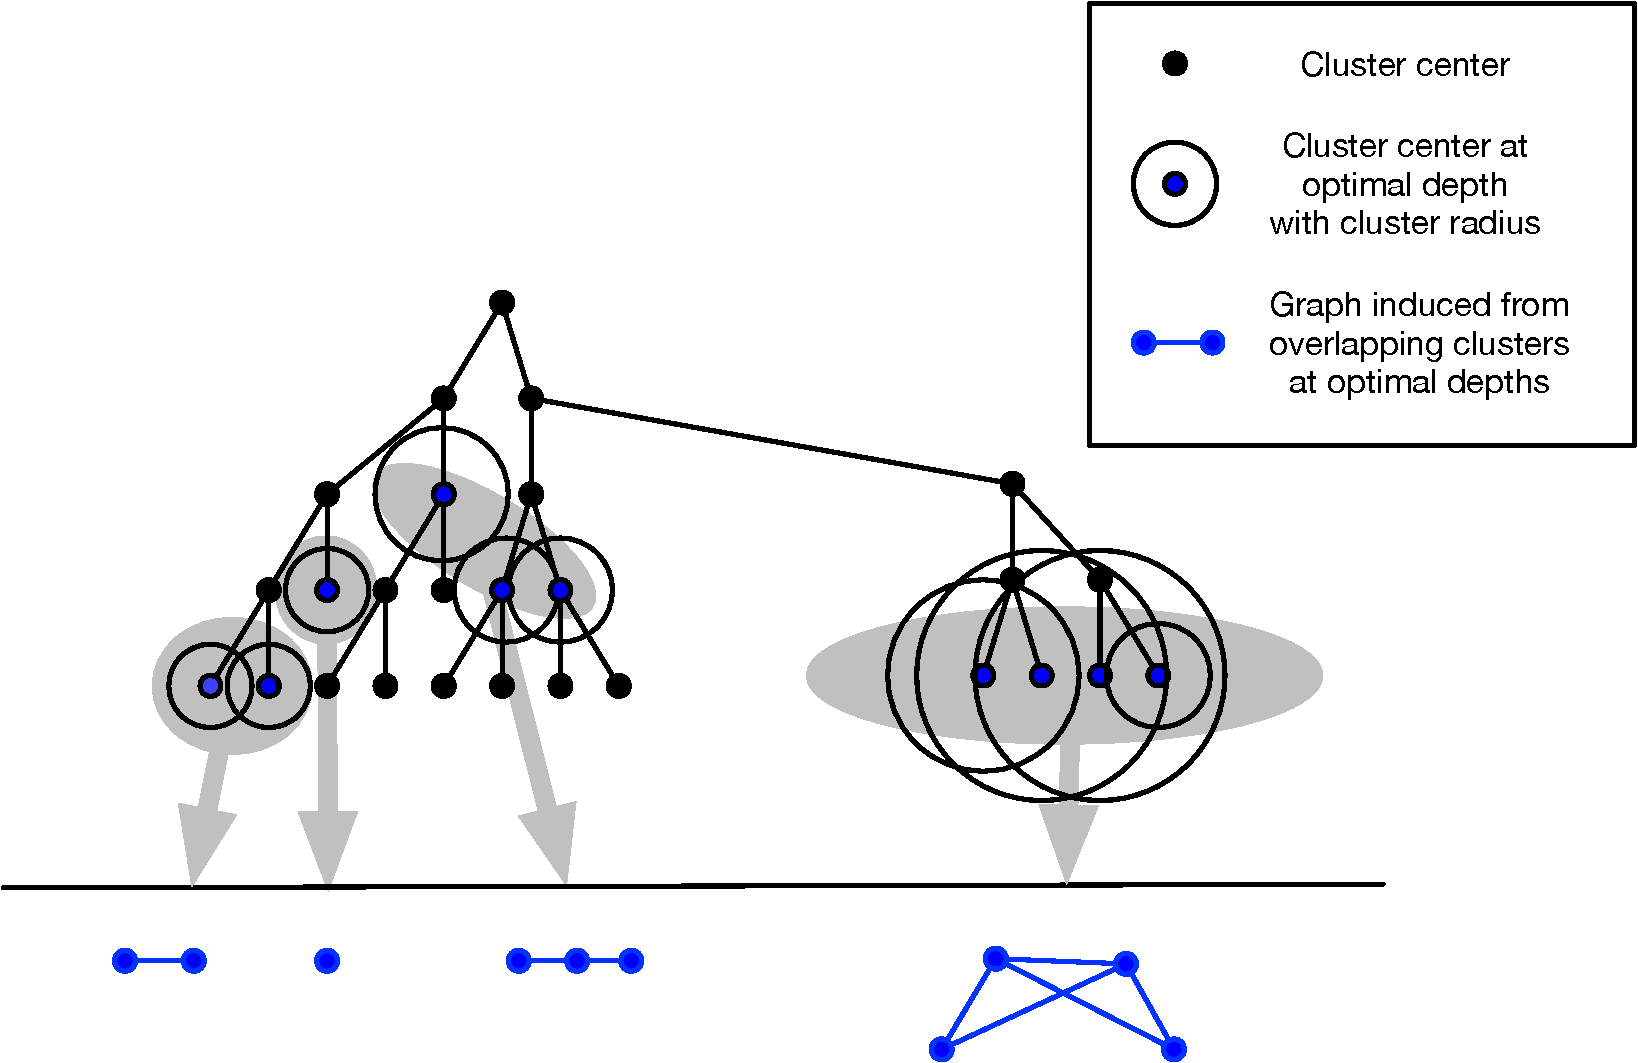
\includegraphics[width=2.5in]{images/tree-graph.pdf}
    \caption{How CLAM induces a graph from a cluster tree.
        Dots in the tree represent cluster centers;
        blue dots represent cluster centers chosen as graph vertices.
        Circles represent the volume of a cluster (the radius is the distance from the center to the furthest point contained within that cluster).
        Gray arrows point to the induced subgraphs, which are indicated in blue below the horizontal line.}
    \label{fig:methods:graph-generation}
\end{figure}


\subsection{Individual Algorithms}
\label{subsec:methods:individual-algorithms}

% TODO change six to five when it's not a lie
Here we describe six simple methods for anomaly detection, each of which uses a graph of clusters from CLAM to calculate an anomalousness score for each datapoint.
For each algorithm, $scores$ is a dictionary of clusters and their outlier scores,
$V$ is the set of clusters in a graph,
$E$ is the set of edges in a graph, and
the cardinality of a cluster $c$ is denoted by $|c|$, the number of points in that cluster.
The key to an effective ensemble method is that each component algorithm contributes a unique inductive bias~\cite{chen2017outlier}.
For each algorithm described below, we note the intuition behind its contribution to the ensemble.

\subsubsection{Relative Cluster Cardinality}
We measure the anomalousness of a point by the cardinality of the cluster that the point belongs to relative to the cardinalities of the other clusters.
Points in the same cluster are considered equally anomalous and points in clusters with lower cardinalities are considered more anomalous than points in clusters with higher cardinalities.
The algorithm is defined in Algorithm~\ref{alg:rclc}.
The time complexity is $\mathcal{O}(|V|)$.

\begin{algorithm}[h]
    \caption{Relative Cluster Cardinality}
    \label{alg:rclc}
\begin{algorithmic}[1]
    \REQUIRE $G$, a graph
    \FOR {cluster $c \in G$}
    \STATE $scores[c] \gets -|c|$
    \ENDFOR
\end{algorithmic}
\end{algorithm}

\subsubsection{Relative Component Cardinality}
We use the usual definition of connected components:
no two nodes from different components have an edge between them, and
every pair of nodes in the same component has a path connecting them.
Consider the relative cardinalities of each component in much the same way as we considered the relative cardinalities of clusters in the relative cluster cardinality method.
Points in clusters (vertices) in smaller components are considered more anomalous than those in larger components,
and points in clusters in the same component are considered equally anomalous.
The algorithm is defined in Algorithm~\ref{alg:rcc}.
This algorithm first finds the components of the graph, so its time complexity is $\mathcal{O}(|E| + |V|)$.

\begin{algorithm}[h]
    \caption{Relative Component Cardinality}
    \label{alg:rcc}
\begin{algorithmic}[1]
    \REQUIRE $G$, a graph
    \FOR {component $C \in G$}
        \STATE $scores[C] \gets -|C|$
    \ENDFOR
\end{algorithmic}
\end{algorithm}

\subsubsection{Graph Neighborhood}
Given the graph with clusters and edges, we consider the number of clusters reachable from a starting cluster within a given graph distance $k$.
We call this number the \textit{graph-neighborhood} of the starting cluster.
With $k$ small compared to the diameter of the graph, we consider the relative sizes of graph-neighborhoods of the clusters.
Points in clusters with small graph-neighborhoods are considered more anomalous than points in clusters with large graph-neighborhoods.
The algorithm is defined in Algorithm~\ref{alg:gns}.
This algorithm is dominated by computing the eccentricity of each cluster, so its time complexity is $\mathcal{O}(|E| \cdot |V|)$.

\begin{algorithm}[h]
    \caption{Graph Neighborhood}
    \label{alg:gns}
\begin{algorithmic}[1]
    \REQUIRE $G$, a graph
    \REQUIRE $f \in \mathbb{R}$ in the range $(0,1]$ ($0.25$ by default).
    \FOR {cluster $c \in G$}
        \STATE $e_c \gets$ the eccentricity of $c$
        \STATE $s \gets e_c \cdot f$
        \STATE perform a breadth-first traversal from $c$ with $s$ steps
        \STATE $v \gets$ the number of unique clusters visited by the traversal
        \STATE $scores[c] \gets -v$
    \ENDFOR
\end{algorithmic}
\end{algorithm}

\subsubsection{Child-Parent Cardinality Ratio}
\label{subsubsec:methods:individual-algorithms:cpcr}
As described in Section~\ref{subsubsec:methods:clam:clustering}, the partition algorithm used in clustering splits a cluster into two children.
If a child cluster contains only a small fraction of its parent's points (thus, the other child has the majority), then we consider the points in that first child cluster to be more anomalous.
These child-parent cardinality ratios are accumulated for each point down its branch in the tree, terminating when the child cluster is a node in the induced graph.
Points with a low value of these accumulated ratios are considered more anomalous than points with a higher value.
The algorithm is defined in Algorithm~\ref{alg:cpcr}.
Unlike other CHAODA algorithms, this one accumulates parent scores into the children.
The time complexity of calculating the ratios is $\mathcal{O}(|V|)$ at clustering time, which is amortized over scoring the points;
the time complexity of scoring a point is $\mathcal{O}(1)$.

\begin{algorithm}[h]
    \caption{Child-Parent Cardinality Ratio}
    \label{alg:cpcr}
\begin{algorithmic}[1]
    \REQUIRE $G$, a graph
    \FOR {cluster $c \in G$}
        \STATE $p \gets$ the parent cluster of $c$
        \STATE $scores[c] \gets \frac{|p|}{|c|} + scores[p]$
    \ENDFOR
\end{algorithmic}
\end{algorithm}

\subsubsection{Random Walks}
We perform long random walks on each component of a graph and count the number of times that each cluster was visited.
We consider the relative visitation counts among the clusters to be inversely related to their anomalousness.
The least visited clusters are the most anomalous, and the most visited clusters are the least anomalous.
The algorithm is defined in Algorithm~\ref{alg:rw}.
This algorithm is dominated by the computation of the transition matrix for the graph.
Its worst-case time complexity is $\mathcal{O}(|V|^2)$, but is often better because the transition matrix is computed separately for each component in the graph.
Importantly, and distinct from the algorithm described in \ref{subsubsec:methods:individual-algorithms:sp}, this approach uses the distance between two cluster centers to determine the random walk, so a closed-form convergent solution cannot be used.

%% NAJIB I don't think the algorithm description reflected the edge weights!
%% I have tweaked it; please check.

\begin{algorithm}[h]
    \caption{Random Walks}
    \label{alg:rw}
\begin{algorithmic}[1]
    \REQUIRE $G = (V,E)$, a graph
    \STATE Initialize $v[c] \gets 0 \ \forall c \in G$
    \FOR {cluster $c \in G$}
        \STATE $c' \gets c$
        \FOR{$i=1$ {\bfseries to} $10 \cdot |V|$}
            \STATE $c' \gets n(d),$ a random neighbor of $d$ chosen with probability inversely proportional to the distance between d and n(d)
            \STATE increment $v[c']$
        \ENDFOR
    \ENDFOR
    \FOR {cluster $c \in G$}
        \STATE $scores[c] \gets -v[c]$
    \ENDFOR
\end{algorithmic}
\end{algorithm}

\subsubsection{Stationary Probabilities}
\label{subsubsec:methods:individual-algorithms:sp}
We compute the transition probability matrix of each component of a graph that contains at least two clusters.
We then compute successive squares of this matrix.
This process will eventually converge as long as the graph is connected and aperiodic~\cite{levin2017markov}; we find this convergent matrix.
We consider the sum of the values along a row to be inversely related to the anomalousness of the respective cluster.
The algorithm is defined in Algorithm~\ref{alg:sp}; it describes the stationary probabilities for an \emph{unweighted} representation of the graph, distinguishing it from the random walk method.
%% NAJIB IS THIS CORRECT?
This algorithm is dominated by the computation of a separate matrix for each component in the graph.
Its worst-case time complexity is $\mathcal{O}(|V|^2)$, but is often better in practice.

\begin{algorithm}[h]
    \caption{Stationary Probabilities}
    \label{alg:sp}
\begin{algorithmic}[1]
    \REQUIRE $G$, a graph
    \FOR {component $C \in G$}
        \STATE $M \gets$ the transition matrix for $C$
        \REPEAT
            \STATE $M \gets M^2$
        \UNTIL $M$ converges
        \FOR {cluster $c \in C$}
            \STATE $s \gets $ the row from $M$ corresponding to $c$
            \STATE $scores[c] \gets -\Sigma(s)$ 
        \ENDFOR
    \ENDFOR
\end{algorithmic}
\end{algorithm}


\subsection{Ensemble}
\label{subsec:methods:ensemble}

% TODO talk about inductive bias (NOAH) once all algorithms are in place (waiting on Najib)

Given a dataset and a list of distance functions for the dataset, we start by building a CLAM tree for each distance function on the dataset.
We extract the parent-child ratios and the exponential moving averages of those ratios for each cluster in each tree.
Given the set of models learned from the training datasets described in Section~\ref{subsec:methods:induced-graphs}, we use each model to rank every cluster, normalized by cardinality.
The highest ranked clusters from each tree are then used to build a graph.
This gives us one graph for each combination of individual algorithm, meta-ML model, and distance function used.
We used the six individual algorithms described in~\ref{subsec:methods:individual-algorithms}, three means (arithmetic, geometric, and harmonic), two meta-ML models (linear regression and regression trees), and two distance metrics ($L1$-norm and $L2$-norm);
thus, we have upto $72$ graphs for each dataset.

Each graph is then used with its corresponding individual algorithm to calculate an outlier score for each point in the dataset.
These outlier scores are then combined into an ensemble by simply taking the mean of all the scores for each point.
We present the AUC scores from this ensemble in Section~\ref{sec:results}.

\subsubsection{Normalization}
\label{subsubsec:methods:normalization}

The individual algorithms described in~\ref{subsec:methods:individual-algorithms} produce outlier scores for each cluster, rather than for each point.
We remedy this by assigning to each point the score of the cluster to which it belongs.
Since our graphs guarantee that each point is in exactly one cluster and that every point from the dataset is accounted for, this assigns an outlier score to each point in a dataset.
However, the individual methods still produce scores with a wide range of values.
The only common feature among these scores is that low scores correspond to inliers and high scores correspond to outliers.
Therefore, we cannot directly compare scores across methods, which is needed for ensemble methods.
Thus, we normalize to the range $[0, 1]$, using gaussian normalization~\cite{kriegel2011interpreting} as defined in Algorithm~\ref{alg:normalization}.
We include sigmoid and min-max normalization as options in our implementation.

\begin{algorithm}[h]
    \caption{Gaussian Normalization}
    \label{alg:normalization}
\begin{algorithmic}[1]
    \REQUIRE $X$, a dataset
    \REQUIRE $S$, a set of outlier scores for each point in $X$
    \STATE $erf: x \mapsto \frac{2}{\sqrt{\pi}} \int_{0}^{x} e^{-u^2} \,du $
    \STATE $\mu \gets mean(S)$
    \STATE $\sigma \gets std(S)$
    \FOR {point $p \in X$}
        \STATE $S[p] \gets \frac{1}{2} \Big( 1 + erf \big(\frac{S[p] - \mu}{\sigma \cdot \sqrt{2}}\big) \Big) $
    \ENDFOR
\end{algorithmic}
\end{algorithm}

\subsubsection{A Note on Runtime Performance}

During testing, we noticed that even though we often see $|V| \ll n $, where $n$ is the number of points in the dataset and $V$ is the set of vertices in a graph, the more expensive methods from~\ref{subsec:methods:individual-algorithms} were prohibitive.
We remedy this by only running the expensive algorithms, i.e.\ graph neighborhood size, random walks, and stationary probabilities, when $|V| < max(128, \lfloor \sqrt n \rfloor)$.
We compared the effect on AUC of using this threshold and present the results in Table~\ref{table:results:test-performance} under the CHAODA-fast and CHAODA rows.
CHAODA-fast exhibits comparable accuracy to CHAODA, so we
set CHAODA-fast as the default in our implementation.


\subsection{Datasets}
\label{subsec:methods:datasets}

We sourced 24 datasets from Outlier Detection Datasets (ODDS)~\cite{rayana2016odds}, for training CHAODA and testing its performance.
All of these datasets were adapted from the UCI Machine Learning Repository (UCIMLR)~\cite{UCIMLR}, and were standardized by ODDS for benchmarks on anomaly and outlier detection.

Of these 24 datasets, we selected six at random for training CHAODA: annthyroid, mnist, pendigits, satellite, shuttle, and thyroid.
The remaining datasets were used to benchmark the performance of CHAODA\@.
We benchmarked CHAODA 30 times with the same split of test and training datasets, with different random seeds for CLAM clustering and CHAODA's random walk algorithm.
We provide more details on the datasets, including size, dimensionality, and fraction of outliers, in the Supplement.
All benchmarks were conducted on a 28-core Intel Xeon E5-2690 v4 2.60GHz, 512GB RAM and CentOS 7 Linux with kernel 3.10.0-1127.13.1.el7.x86\_64 \#1 SMP and Python 3.6.8.

Note that CHAODA is an unsupervised algorithm.
As such, we compare only against other unsupervised algorithms.
We compared against $18$ unsupervised algorithms collected in the pyOD suite~\cite{zhao2019pyod} and Scikit-Learn~\cite{pedregosa2011scikit}, as well as RS-Hash~\cite{sathe2016subspace}.
A supervised version of CHAODA is possible future work which we will compare against supervised methods such as REPEN~\cite{pang2018learning}.